%
% fig-exzess.tex
%
% (c) 2025 Prof Dr Andreas Müller
%
\begin{figure}
\centering
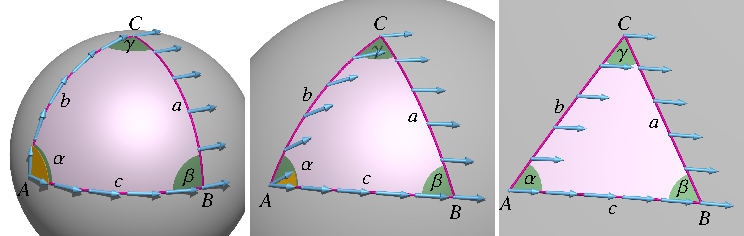
\includegraphics{chapters/110-kruemmung/images/exzess.pdf}
\caption{Der Paralleltransport eines Tangentialvektors um ein 
sphärisches Dreieck führt wegen der Krümmung der Kugeloberfläche
zu einer Drehung des Vektors um den orangen Winkel beim Punkt $A$.
Für kleine Dreiecke bzw.~grosse Kugelradien nähert sich das
Dreieck einem ebenen Dreieck an und die Drehung wird sehr klein.
\label{buch:kruemmung:fig:exzess}}
\end{figure}
